\documentclass{hbrs-ecta-report}

\usepackage{float}
\usepackage{placeins}
\usepackage{ngerman}
%\usepackage[utf8]{inputenc}
\usepackage{fontspec}
\begin{document}

\conferenceinfo{H-BRS}{2017}

\title{Neuroevolution: Recurrent Neural Network}
\subtitle{}

\numberofauthors{2}
\author{
\alignauthor
Tim L"ugger, Jan Urfei
}

\date{today}
\maketitle
\begin{abstract}
Aufgabe:Implementieren Sie ESP. Nutzen Sie die Datei trainingData.mat um die Herzfrequenz aus der Laufgeschwindigkeit und der Zeit vorherzusagen. Lösen Sie außerdem das TwoPoleBalancing- Problem mit ESP.
\end{abstract}

\section{Recurrent Neural Network}
Ein Rekurrentes Neuronales Netzwerk besteht aus einem vollvermaschtem Neuronalen Netz, das an gewissen Knoten einen Input bekommt, und an definierten Knoten einen Output liefert.
Als Algorithmus liegt im Prinzip für jeden Knoten ein genetischer Algorithmus vor. Jeder Knoten hat von allen anderen Knoten Kanten, die zu ihm führen, mit einem speziellen Gewicht. Man bildet pro Knoten einen eigene Subpopulation. Ein Genom aus der Population sieht so aus, dass dort die Kantengewichte als Vektor aufgeschrieben sind. Für die Berechnung der Fitness lässt man jedes Genom aus jeder Subpopulation zufällig mehrmals mit anderen Genomen aus den anderen Populationen ein Netz bilden, durch das man dann den Trainingsdatensatz schickt. Die Fitness die sich daraus ergibt wird den teilnehmenden Knoten zugewiesen. Da jeder Knoten mehrmals daran teilnimmt bildet man nachher den Mittelwert und erhält so einen speziellen Fitnesswert für das eine Genom.\\
Wenn das passiert ist, wird ein normaler Genetischer Algorithmus angewendet. Man behält sich die Elite in der Population und generiert sich mittels Crossover und Mutation neue Genome, die dann in die nächste Epoche mit einfließen. 


\section{Herangehensweise}
 
 Das erste was wir in unserem Algorithmus gemacht haben ist, aufzuteilen, welche Daten Trainingsdaten sind und welche Daten zum Test genommen werde. Die ersten 10 Trainingsläufe aus $train_data$ sind bei uns die Trainingsdaten. 
Als nächstes haben wir alle Parameter die man verändern kann nach oben gezogen. Das sind einmal die Parameter über die Anzahl der Knoten des Netzwerks. Und dann noch die Parameter die für den genetischen Teil gebraucht werden, wie z.B. die Mutationsrate.\\
Nachdem das alles festgelegt ist lassen wir zufällige Startpopulationen erzeugen. Jetzt folgen ganz viele ineinander verschachtelte Schleifen. 
Die äußerste Schleife dient dazu den Kompletten Trainingsdurchlauf mehrmals zu wiederholen. Sie stellt sozusagen die verschiedenen Epochen dar. Die zweite Schleife sorgt dafür, dass alle Trainingsläufe durchlaufen werden.
Da wir alle Genome mehrmals mit verschiedenen anderen Genomen an einem Netzwerk teilnehmen lassen wollen um sie nachher bewerten zu können brauchen wir noch eine Schleife, die dafür verantwortlich ist, dass jedes Genom X mal an einem Netzwerk teilnimmt. Damit auch garantiert ist, dass jeder Knoten X mal teilnimmt lassen wir jede Subpopulation permutieren und nehmen dann aus jeder Subpopulation die ersten Genome und danach die zweiten usw. Dieser Vorgang benötigt ebenfalls eine Schleife. Die letzte Schleife darin braucht man, um realisieren zu können, dass jede Messreihe aus dem Trainingslauf der Reihe nach durchgegangen wird.\\
Unsere Gewichtsmatrix setzt sich aus einem Genom pro Subpopulation zusammen. Die Eingabe wird dann mit den aktuellen Zuständen des Netzwerkes verknüpft und dann mit der Gewichtsmatrix multipliziert. So kommt man zu dem nächsten Zustand des Netzes. Als Aktivierungsfunktion der einzelnen Neuronen verwenden wir die $tanh()$ Funktion.  \\
Die Fitness wird nach jeder Messreihe bestimmt und zwar durch die Funktion $ 0.5 * (target-outpu)^2 $. Diese Fehler werden dann aufaddiert und den Teilnehmenden Knoten zugewiesen. Da die Trainingsläufe unterschiedlich lang sind. Teilen wir die Summe noch durch die Länge der Trainingsläufe um die Ergebnisse zu normieren. Da die Knoten ja insgesamt auch zehnmal bewertet werden teilen wir die Fitness auch noch durch 10 am Ende. Das wäre nicht zwingend notwendig, hat dann aber eine semantisch stärkere Bedeutung. 
Nachdem die Fitness von einem Knoten dann feststeht kommt ein genetischer Algorithmus der pro Subpopulation genauso funktioniert, wie unser Simple Genetic Algorithm aus der vorangegangenen Übung.


\section{Unsere Ergebnisse}

\subsection{Heart Rate}

Das Diagramm in Figure \ref{fig:Error} ist mit einer Subpopulationsgröße von 15, einer Mutationsrate von 0.5, einer Crossoverrate von 0.1 und einer Standardabweichung von 0.01 entstanden.
Als Mutation wird jedes eingehende Kantengewich um einen normalverteilten Zufallswert erhöht. 
Bei dem Crossover erhält das Genom, jedes Kantengewicht von einem zufällig ausgewähltem anderen Genom.

\begin{figure}[h!]
	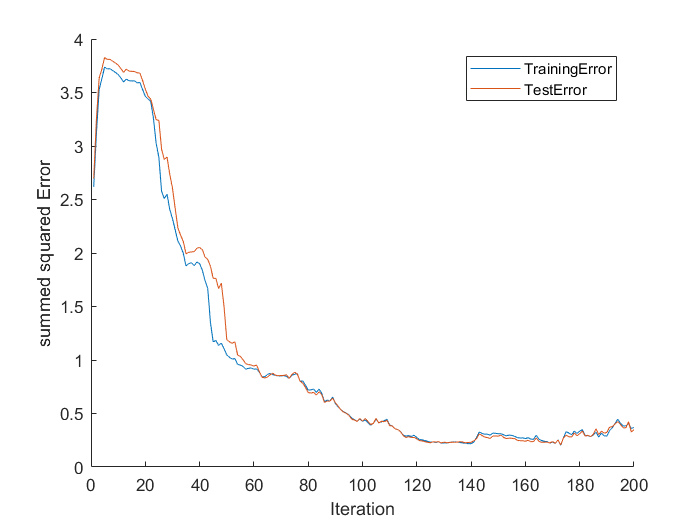
\includegraphics[width=\linewidth]{img/TrainingTestError}
	\caption{Fehler der besten Genome der Populationen über die Epochen}
	\label{fig:Error}
\end{figure}
\FloatBarrier

Es wird sehr stark deutlich, dass der Fehler anfangs sehr stark runter geht und dann bei ca 0.3 stagniert. Das kann auch an der Leistungssteigerung liegen, die der Proband von den Messdaten durchlaufen hat, da die Trainingsdaten ja wieder von vorne gelernt werden, wenn einmal die 10 durch sind. Auch ein Problem sind die 0 Werte am Anfang einer Messreihe, die in den unterschiedlichen Messreihen nie gleichlang sind. 

\subsection{Pole Balancing} 
Beim Pole Balancing gestaltete sich die Anwendung von ESP schwieriger. Durch das aufwendiger Training war eine Auswahl geeigneter Hyperparamter ebenfalls aufwendig.
In Figure 2 erkennt man, dass die Fitness zwar ansteigt, aber stark schwankend ist sowie nach vielen Iterationen abflacht oder sogar abfällt. Die selbe Beobachtung konnten wir bei unterschiedlichen Hyperparametern machen.

Eines der besseren Ergebnisse erreichte stabile ~200 Schritte mit Ausreißern bis <450. Figure 3

Da wir wissen, dass ESP für diese Aufgabe 10000 Schritte schaffen sollte, schließen wir darauf, dass ein Fehler in unserer Implementierung vorliegt, die Hyperparameter falsch gewählt wurden und/oder die Trainingszeit nicht ausgereicht hat.


\begin{figure}[h!]
	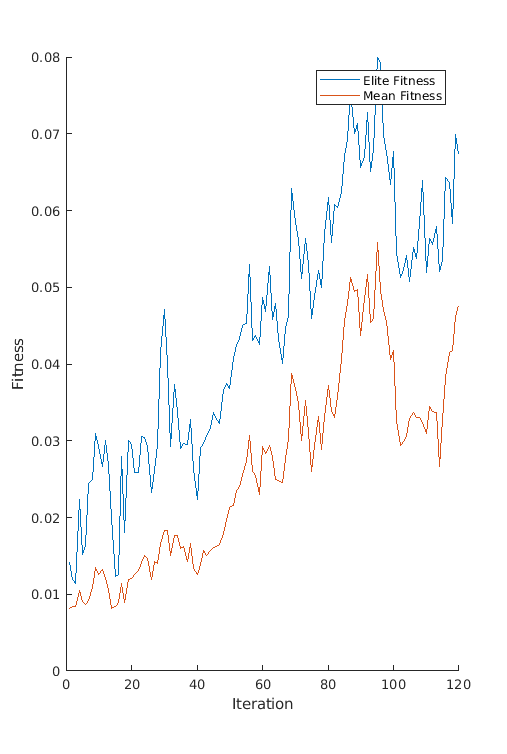
\includegraphics[width=0.8\linewidth]{img/poleFitness}
	\caption{Durchschnittliche Fitness sowie Fitness des Besten Netzes pro Iteration}
	\label{fig:fitness}
\end{figure}

\begin{figure}[h!]
	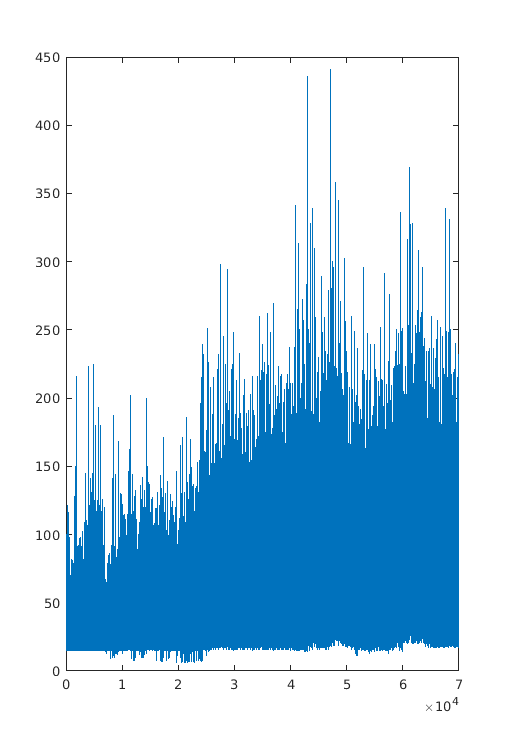
\includegraphics[width=0.8\linewidth]{img/poleSteps}
	\caption{Anzahl der Schritte die nach jeder Ausführung der Simulation erreicht wurden}
	\label{fig:steps}
\end{figure}

\end{document}
}